\chapter*{Introduction}


\section{Objectifs}

L'objectif du cours est l'étude des fonctions de la variable complexe  prenant leurs valeurs dans le plan complexe. A la fin de cet enseignement, vous devrez :
\begin{itemize}
    \item Connaître et savoir appliquer la notion de différentiabilité dans $\C$ et les règles de calcul associées, 
    \item Connaître et savoir appliquer dans des cas relativement simples l'intégration le long de chemins, en particulier par le théorème des résidus, qui s'applique au calcul d'intégrales semi-convergentes, 
    %\item Connaître et savoir expliquer l'intérêt des surfaces de Riemann,  
    \item Connaître la définition et savoir appliquer la transformation de Laplace dans les sens direct et inverse
\end{itemize}

\section{Pourquoi ?}
Ce domaine peut paraître d'une grande abstraction, et l'étudiant ingénieur pourrait se demander ce qu'un tel enseignement vient faire dans son cursus. En réalité, la théorie des fonctions de la variable complexe permet de résoudre de nombreux problèmes, dans des domaines très divers. Nous pouvons notamment citer :
\begin{itemize}
    \item la mécanique des fluides, en particulier l'aide au calcul d'un profil d'une aile d'avion par la \emph{transformation de Joukovsky} (on pourra consulter le site \linebreak\texttt{airfoil.dimanov.com} 
    qui propose une applet interactive) qui a été beaucoup utilisée du début du XXème siècle,
    \item l'électromagnétisme : une fonction $\C$-dérivable a comme parties réelle et imaginaire des fonctions \textbf{harmoniques} (leur laplacien est nul),
    \item l'automatique, avec la transformation de \emph{Laplace},
    \item la cartographie, avec les projections \emph{stéréographique}, \emph{Mercator} et \emph{Lambert}. 
\end{itemize} 
\vspace{0.1in} 

Plusieurs points de vue permettent d'appréhender les fonctions de la variable complexe. Par exemple, on pourra interpréter toute fonction $f$ comme une règle de transformation du plan complexe~; au point $z \in \C$ est associé le point $w = f(z) \in \C$. Cette vision géométrique, outre le fait qu'elle offre une approche très visuelle de ces fonctions, est très importante de point de vue théorique. Elle dérive historiquement des problèmes de cartographie de la Terre qui furent étudiés par Gauss, Mercator, Lambert, Euler et Lagrange. Le problème consistait à représenter la sphère sur le plan en demandant par exemple~:
\begin{itemize}
    \item la préservation des aires (carte équivalente), 
    \item la préservation des angles (carte conforme), 
    \item la préservation des distances (carte équidistante),
    \item la préservation de certaines courbes privilégiées (carte orthodromique, carte loxodromique).
\end{itemize} 
\vspace{0.1in} 

Rappelons l'impossibilité d'appliquer homéomorphiquement \textit{(de façon bijective, continue et de réciproque continue)} la sphère sur le plan, la sphère étant compacte à la différence du plan. Contourner ce défaut nécessite de compacifier le plan en ajoutant un point dit "à l'infini". L'espace ainsi obtenu est alors homéomorphe à la sphère, dite sphère de Riemann, et cet homéomorphisme est connu sous le nom de projection stéréographique. Il sera étudié de façon explicite dans la section \ref{CompacC}
%Nous verrons que pour étudier les transformations du plan, il est souvent plus simple de travailler sur la sphère de Riemann, car en particulier les droites du plan correspondent aux cercles passant par le pôle Nord de la sphère de Riemann, image du point à l'infini. Ainsi, aux transformations de la sphère de Riemann qui préservent les cercles correspondent les transformations du plan qui préservent la famille des cercles et des droites~; par exemple à une translation du plan transportant l'origine au point $P$ correspond la rotation de la sphère de Riemann transportant le pôle Sud en l'image du point $P$.   





\section{Contenu}
Nous nous intéresserons aux fonctions complexes dites \emph{holomorphes} qui correspondent aux transformations conformes du plan, c'est à dire aux transformations préservant les angles, ou encore \emph{semblable en ses parties infiniment petites}. Ici le terme \emph{semblable} doit être interprété dans le sens géométrique de préservation de la forme~: par exemple l'image d'un triangle infiniment petit sera un triangle semblable.
\vspace{0.1in} 

Les applications globalement semblables dans le plan sont les similitudes directes et indirectes, nous verrons que les fonctions holomorphes sont des fonctions différentiables dont la différentielle est une similitude directe du plan. Or les similitudes du plan sont les applications qui préservent la famille des cercles et des droites du plan, elles correspondront donc aux transformations de la sphère de Riemann qui préservent les cercles et laissent fixe le pôle Nord. Aux transformations (bijectives) de la sphère de Riemann ne fixant le pôle Nord correspondent, via la projection stéréographique, les transformations du plan appelées \emph{transformations de Möbius}.

\vspace{0.1in} 

Ce cours ne fait qu'introduire à l'analyse complexe, il n'aborde pas en particulier l'étude des transformations conformes du plan, le lien entre la physique et les fonctions complexes et surtout le théorème de Riemann qui stipule que tout ouvert de $\C$, avec $U \neq \C$ est conformément équivalent au disque unité ; pour plus de détails consulter par exemple \cite{nehari2012conformal}. 

\vspace{0.1in} 

Dans une première partie nous présenterons quelques notions de topologie utiles pour la suite. Dans une seconde partie, nous définirons les fonctions holomorphes et énoncerons les conditions de Cauchy-Riemann qu'elles devront satisfaire. Dans le chapitre 3, nous expliquerons comment intégrer une fonction complexe le long d'un chemin, regroupant sous une seule intégrale la notion de travail et de flux d'un champ de vecteurs, notions très utiles en physique. Le chapitre 4 énoncera le théorème des résidus, théorème fondamental par son usage pour le calcul d'intégrale le long d'un contour fermé mais aussi pour son lien entre l'intégration et la géométrie du plan complexe. Enfin, le chapitre 5 propose une introduction à la notion de surface de Riemann; elle a été introduite par Bernhard Riemann pour prendre en compte les singularités et les complications topologiques qui accompagnent certains prolongements analytiques de fonctions holomorphes. Un exemple est la sphère de Riemann, mais il en existe beaucoup d'autres, par exemple la surface associée à la fonction logarithme complexe ou racine n-ième. Pour une présentation plus complète de ce sujet, le lecteur pourra consulter \cite{de2010uniformisation}.




%\newpage
%\section{Sphère de Riemann} 

%\subsection{Sphère de Riemann}

%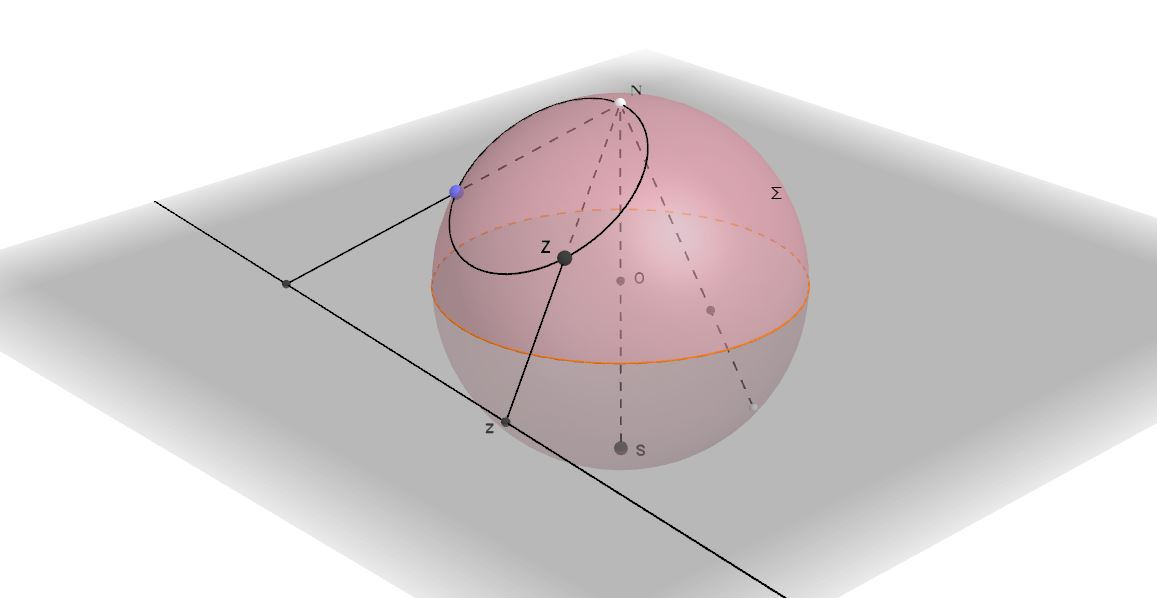
\includegraphics[scale=0.3]{stereo_proj.png}















%Le fait d'adjoindre à $\C$ un point à l'infini permet d'obtenir un espace  $\overline{\C}$ compact isomorphe à la sphère de $\R^3$. Le moyen de se convaincre de se résultat est de considérer la projection stéréographique du plan complexe sur la sphère unité.  

%\begin{figure}
%\label{fig:sphereRiemann}
%\begin{center}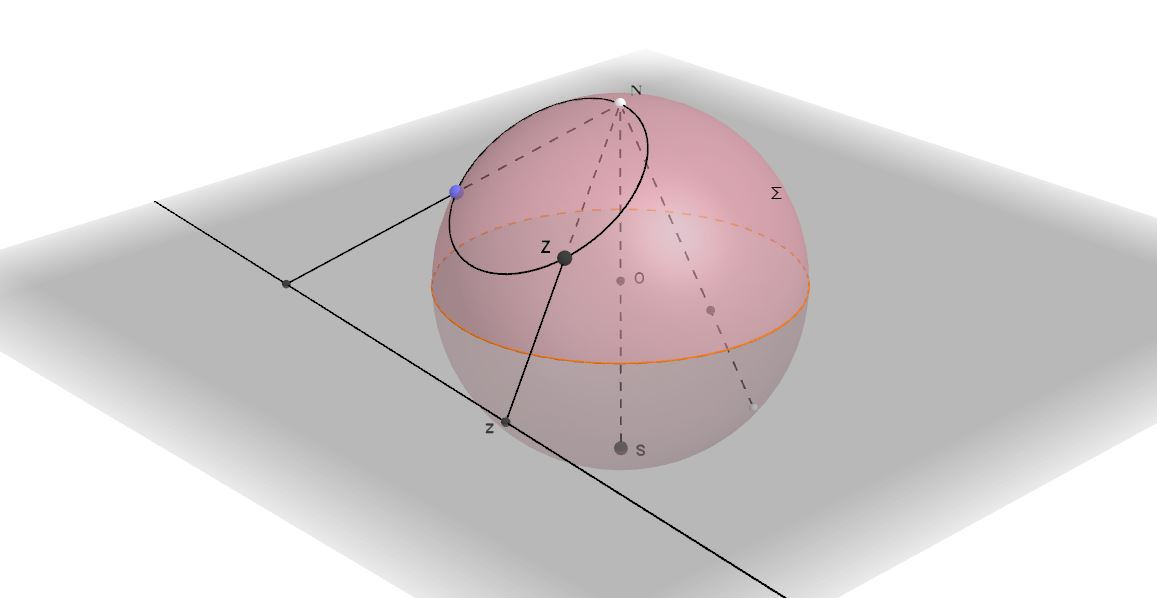
\includegraphics[scale=0.5]{stereo_proj}
%\end{center}
%\caption{Sphère de Riemann}
%\end{figure}

%Considérons dans $\R^3$, la sphère $\Sigma$ de rayon l'unité et centrée en l'origine (cf. figure~\ref{fig:sphereRiemann}). On projette le point d'affixe $z \in \C$ sur la sphère en considérant l'intersection $Z$ de la droite reliant $z$ au point $N=(0,0,1)$, appelé pôle Nord, avec la sphère $\Sigma$. Réciproquement un point $Z$ de la sphère est transformé en le point $z$, intersection de la droite passant par le pôle Nord et le point $Z$ avec le plan $\C$. Nous observons que le point $S=(0,0,-1)$, appelé pôle Sud est transformé en l'origine $O$ et que les points du cercle unité dans $\C$ sont invariant. De plus, l'image de toute calotte sphérique centrée en $N$ est un voisinage du point à l'infini. Il est donc naturel de considérer le pôle Nord comme le point à l'infini, et la transformation décrite est une bijection entre $\overline{\C}$ et la sphère $\Sigma$. Cette transformation est appelée projection stéréographique et la sphère $\Sigma$ est appelée sphère de Riemann. 

%La transformation stéréographique associe à tout point $\hat{Z}=(X,Y,Z)$ de la sphère, lorsque $Z \neq 1$, le point $z=\frac{X+i Y}{1-Z}$, où bien si $\hat{Z} = (\phi,  \theta)$ (en coordonnées sphériques), le point $z= \cot (\phi/2) e^{i \theta}$.   



%\section{Exercices complémentaires}

